\documentclass[11pt,letterpaper]{article}
\usepackage[lmargin=1in,rmargin=1in,tmargin=1in,bmargin=1in]{geometry}
\usepackage{../style/homework}
\usepackage{../style/commands}
\setbool{quotetype}{true} % True: Side; False: Under
\setbool{hideans}{true} % Student: True; Instructor: False

% -------------------
% Content
% -------------------
\begin{document}

\homework{11: Due 11/06}{Learning is not attained by chance; it must be sought for with ardor and attended to with diligence.}{Abigail Adams}

% Problem 1
\problem{10} Find the equation of the line plotted below.
	\[
	\fbox{
	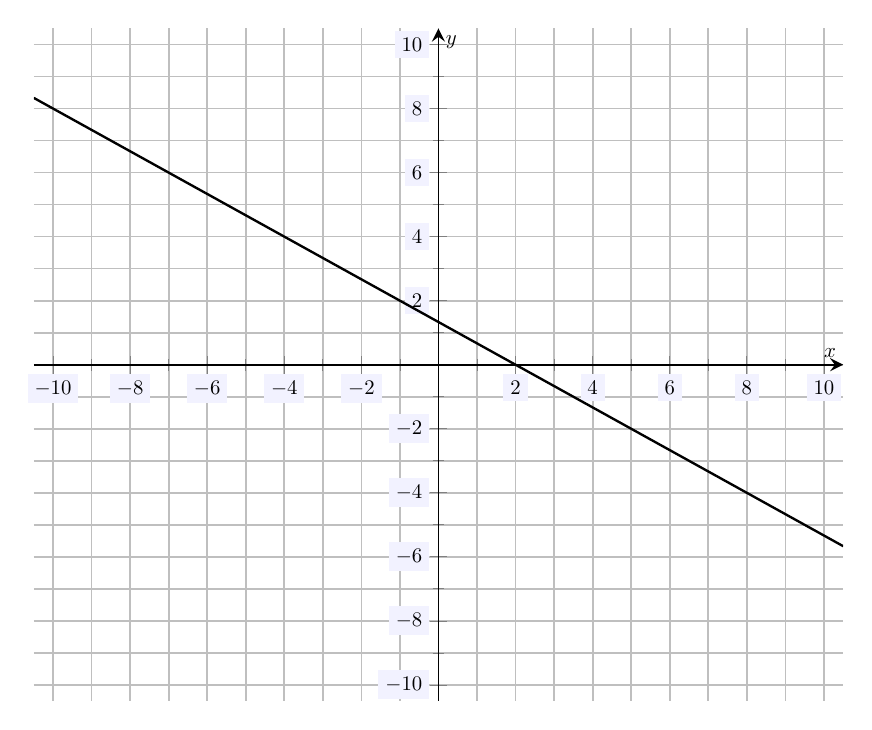
\begin{tikzpicture}[scale=1.5,every node/.style={scale=0.5}]
	\begin{axis}[
	grid=both,
	axis lines=middle,
	ticklabel style={fill=blue!5!white},
	xmin= -10.5, xmax=10.5,
	ymin= -10.5, ymax=10.5,
	xtick={-10,-8,-6,-4,-2,0,2,4,6,8,10},
	ytick={-10,-8,-6,-4,-2,0,2,4,6,8,10},
	minor tick = {-10,-9,...,10},
	xlabel=\(x\),ylabel=\(y\),
	]
	\addplot[line width= 0.02cm,samples=2,domain= -10.5:10.5] ({x},{4/3 - 2/3*x});
	\end{axis}
	\end{tikzpicture}
	}
	\] 



\newpage



% Problem 2
\problem{10} Find the equation of the line containing the point $(-5, 6)$ with slope $-\frac{1}{3}$. 



\newpage



% Problem 3
\problem{10} Find the equation of the line with $x$-intercept 5 and $y$-intercept $-6$. 



\newpage



% Problem 4
\problem{10} Find the equation of the line parallel to the line $\ell(x)= \frac{4 - x}{6}$ whose $x$-intercept is $(9, 0)$. 


\end{document}